\documentclass{article}
\usepackage{ee105}

%% Makes figure labels bold
\usepackage[labelfont=bf]{caption}

\begin{document}
\thispagestyle{plain}

\tutorial{HP 54615B Oscilloscope}

\tableofcontents

\section{Introduction}
The HP54615B is an oscilloscope, used primarily to measure voltages that vary with time. There are two independent in put channels, which can be used simultaneously to measure and compare two waveforms (e.g. input and output waveforms for a filter).

The default mode on the oscilloscope will plot time on the horizontal axis and voltage on the vertical axis. The scaling of each axis can be controlled independently for each input. Scaling can either be done manually or with the ``Auto Scale'' button. There are other modes of operation for the oscilloscope, such as the XY mode in which one channel is plotted against the other in a Voltage-Voltage plot, but in these labs you will primarily use the default mode.

This tutorial starts with quick notes on the most vital information, so if you feel somewhat familiar with oscilloscopes you can check over the quick notes and figure out the details on your own. The later sections include more detailed descriptions of the HP54615B interface and some examples of common measurements.

\section{Quick Notes (to get started fast)}
\begin{itemize}
\item After connecting the probes, try the \textbf{Auto Scale} button. It will generally provide a good axis scaling if the waveform is not too irregular, small, or high-frequency.
\item Each channel has vertical scaling controls to manually set scaling. You can see the current axis scaling at the top-left of the screen (generally in volts per division) and adjust the scaling with the knobs in the ``Vertical'' section. There is one vertical scaling knob per input channel.
\item Measure signals (e.g. $V_{p-p}$) by pressing the appropriate button in the ``Measure'' section of the panel (e.g. \textbf{Voltage}) and then selecting the appropriate value to measure from the menu buttons beneath the screen.
\item Cursors can also be placed with the \textbf{Cursor} button, menu buttons beneath the screen, and the knob next to the \textbf{Cursor} button.
\item AC coupling will remove any DC bias (offset) from the measured signal. Coupling can be selected with the menu buttons beneath the screen.
\item The oscilloscope's ground is \textbf{earth ground}, so the black alligator wires on the oscilloscope probes are connected together. Since the function generator is also earth-grounded, the oscilloscope probe grounds are connected to the function generator ground. To avoid shorts to ground, you should \textbf{always connect the oscilloscope ground clips to the same node}. Do not try to use the probes to measure floating signals (as you can with the DMM).
\end{itemize}

\section{Triggers}
The HP54615B has a ``Trigger'' input section on its interface panel. Triggers are used to synchronize oscilloscope timing with an external signal so that measurements can be taken at the correct time. For example, to capture a single voltage pulse, one might use a trigger input to signal the oscilloscope to take measurements at the pulse arrival. Triggers can also be used with periodic inputs.

Generally, you will not need to use oscilloscope triggering in these labs.

\section{Interface Details}
The power button is in the lower-left corner of the front panel. 

The oscilloscope screen displays measurement axes. At the top of the screen, vertical and horizontal scaling units are displayed. The default mode will display vertical scaling for each input in volts/div and horizontal scaling in seconds/div, where the corresponding divisions make up the grid of squares on the screen.

The buttons beneath the screen are referred to as ``menu buttons'' or ``context buttons'' in this tutorial. Their functionality changes with other button pushes (e.g. by pushing the \textbf{Measure Voltage} button). Each button's current function is labeled on the screen by the text immediately above the button. These menu buttons are essential to taking measurements and performing more complex functions on the oscilloscope.

This tutorial will describe the sections of the front interface panel in the general order you would consider them to take a waveform measurement after pressing the \textbf{Auto Scale} button. At the end of the tutorial there are examples of common measurement procedures.

There is a photo of the HP54615B front panel in Figure \ref{frontpanel}.

\begin{figure}[!htb]
  \centering
  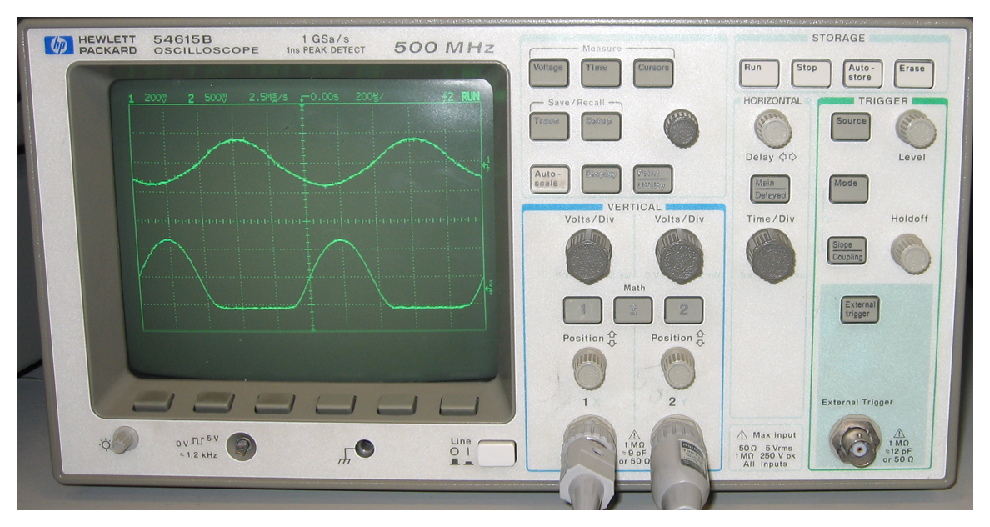
\includegraphics{HP54615B.eps}
  \caption{HP54615B Front Panel}
  \label{frontpanel}
\end{figure}

\subsection{Auto Scale Button}
The \textbf{Auto Scale} button has the oscilloscope ``guess'' a good axis scaling based on the input waveform on each channel. This button is always a good first pass for scaling, and often will be all the scaling that you will need. You can tune the scaling manually with the Vertical and Horizontal controls, described below.

\subsection{Vertical Section}
The vertical controls adjust the scaling and position of each independent channel display. The controls for each channel are aligned vertically with each input port.
\begin{itemize}
\item The \textbf{Volts/Div} knob sets the vertical scaling (vertical zoom) on the display.
\item The ``1'' and ``2'' buttons toggle showing their respective inputs.
\item The position knob controls the voltage offset against the display axes. The horizontal axis does not represent 0 volts, but instead the 0 volt position for each input is designated by a numbered ground symbol on the right of the display. When you adjust the offset with the position knob, you will see the corresponding channel's ground symbol move vertically.
\item The \textbf{Math} button can combine inputs with one of the following arithmetic operators: addition, subtraction, or multiplication. The operation can be selected with the menu buttons beneath the screen after pushing the \textbf{Math} button. 
\end{itemize}

When using the Vertical control section (e.g. after pushing ``1'' or ``2''), the menu buttons beneath the screen show a menu with various options related to the probe inputs. The list below assumes that the ``1'' button has been pushed.
~\\~\\
\textbf{Menu 1}
\begin{itemize}
\item 1: ON/OFF  -  Toggles the display of input 1.
\item Input: \unit{50}{\ohm}/\unit{1}{\mega\ohm}  -  Toggles the input impedance to the channel input. Should usually be set at \unit{1}{\mega\ohm}.
\item Coupling: DC/AC/ground  -  Sets the coupling for the channel input (DC will show both DC and AC values, AC will only give time-varying voltage values and remove any offset, and ground will set it as a virtual ground).
\item BW Lim: Off/On  -  Leave this at default.
\item Vernier: Off/On  -  Leave this at default.
\item Next Menu  -  Go to Menu 2.
\end{itemize}
\textbf{Menu 2}
\begin{itemize}
\item Invert: Off/On  -  Toggles inversion of input signal. Should be Off.
\item Probe: AutoIO  -  Leave this setting on AutoIO.
\item Protect: Off/On  -  Leave this setting On.
\item Previous Menu  -  Go to Menu 1.
\end{itemize}

\subsection{Horizontal Section}
The horizontal axis is the same for both input channels.
\begin{itemize}
\item The \textbf{Time/Div} knob sets the horizontal scaling (horizontal zoom) on the display for both input channels. 
\item Control the horizontal position with the \textbf{Delay} knob.
\end{itemize}

\subsection{Display Button}
By pressing the \textbf{Display} button, the menu buttons beneath the display become the following:
\begin{itemize}
\item Display Mode: Normal/PeakDet/Average  -  The display mode will be used most often, but to average measurements over several samples (useful for noisy signals) use the Average display mode.
\item Average Over: 8/64/256  -  Only visible in Average mode, this button switches between the available sample numbers to average over. For example, to average over 8 samples, push this button until the ``8'' is selected.
\item Vectors: Off/On  -  Leave this setting Off.
\item Grid: Full  -  Leave this setting on Full.
\end{itemize}

\subsection{Measure Section}
The measure section has buttons for \textbf{Voltage}, \textbf{Time}, and \textbf{Cursors}. Cursors are discussed in the next subsection.

To make a voltage measurement on an input signal, press the \textbf{Voltage} button. It will change the menu buttons beneath the screen so that you can select which voltage parameter to measure. Values will be displayed at the bottom of the screen, and automatic cursors will be placed around the selected measurement on the display. Additional measurements will line up at the bottom of the display.

After pressing the \textbf{Voltage} button, the menu buttons beneath the screen become the following:
~\\~\\
\textbf{Menu 1}
\begin{itemize}
\item Source: 1/2  -  Selects the source on which to perform the measurement.
\item Voltage Measurements: $V_{p-p}$/$V_{avg}$/$V_{rms}$  -  Press this button until the intended value to measure is selected.
\item Clear Meas  -  Clear measurements on the bottom of the screen.
\item Next Menu  -  Go to Menu 2.
\end{itemize}
\textbf{Menu 2}
\begin{itemize}
\item Show Meas: Off/On -  Toggle showing measurements.
\item Voltage Measurements: $V_{max}$/$V_{min}$/$V_{top}$/$V_{base}$  -  Press this button until the intended value to measure is selected.
\item Next Menu  -  Go to Menu 3.
\end{itemize}
\textbf{Menu 3}
\begin{itemize}
\item Voltage Measurements: $V_{amp}$/$V_{over}$/$V_{pre}$  -  Press this button until the intended value to measure is selected.
\item Next Menu  -  Go to Menu 1.
\end{itemize}

To make a time measurement on an input signal, press the \textbf{Time} button in the Measure section. It will change the menu buttons beneath the screen so that you can select which time parameter to measure. Values will be displayed at the bottom of the screen, and automatic cursors will be placed around the selected measurement on the display. Additional measurements will line up at the bottom of the display.

After pressing the \textbf{Time} button, the menu buttons beneath the screen become the following:
~\\~\\
\textbf{Menu 1}
\begin{itemize}
\item Source 1/2  -  Selects the source on which to perform the measurement.
\item Time Measurements: Freq/Period/Duty Cy  -  Press this button until the intended value to measure is selected. Duty cycle for a square wave is defined as the percent of the period for which the voltage level is high.
\item Clear Meas  -  Clear measurements at the bottom of the screen.
\item Next Menu  -  Go to Menu 2.
\end{itemize}
\textbf{Menu 2}
\begin{itemize}
\item Show Meas: Off/On  -  Toggle showing measurements.
\item Time Measurements: +Width/-Width/RiseTime/FallTime  -  Press this button until the intended value to measure is selected.
\item Next Menu  -  Go to Menu 3.
\end{itemize}
\textbf{Menu 3}
\begin{itemize}
\item Define Thresholds  -  Set up threshold time values.
\item Define Delay  -  Set up a measurement delay.
\item Measure: Delay/Phase  -  Measure a delay or phase difference between signals.
\item Next Menu  -  Go to Menu 1.
\end{itemize}

\subsection{Cursors}
Cursors are markers that you can place to manually measure quantities on the display axes. For example, you can measure a specific voltage point on the vertical axis with a cursor or measure the voltage difference between two cursors placed on the vertical axis.

After presing the \textbf{Cursor} button, use the menu buttons beneath the sceen to activate a particular cursor. You can use the knob to adjust the position of the cursor manually. Cursor measurements are displayed at the bottom of the screen.

After pressing the \textbf{Cursor} button, the menu buttons beneath the screen become:
\begin{itemize}
\item Source: 1/2  -  Select source on which to place cursor.
\item Active Cursor: V1/V2/T1/T2  -  Select which cursor is adjustable with the knob. There are two voltage cursors and two time cursors for each input. Press this button until the desired cursor is selected, and then use the knob to edit it.
\item Readout: Volts/\%  -  Toggle the readout of the cursor value between volts and percentage (for a voltage cursor). This button allows you to change the time value displayed as for time cursors.
\item Clear Cursors  -  Clear the currently placed cursors and their corresponding measurements from the screen.
\end{itemize}

\section{Examples}
These examples assume you have already turned on the oscilloscope and that the desired signal is either on Channel 1 or both channels.

\subsection{Measuring $V_{p-p}$ of a Waveform}
\begin{enumerate}
\item Press the \textbf{AutoScale} button and adjust the horizontal and vertical scaling so that the wave is visible.
\item Press the \textbf{Voltage} button in the Measure section.
\item Verify that the correct source is selected (1) on the leftmost menu button.
\item Select $V_{p-p}$ from the menu buttons beneath the screen.
\item The $V_{p-p}$ value will be displayed at the bottom of the screen, and the measured peak-to-peak distance will be displayed with two horizontal cursors around the waveform.
\end{enumerate}

\subsection{Measuring Frequency of a Waveform}
\begin{enumerate}
\item Press the \textbf{AutoScale} button and adjust the horizontal and vertical scaling so that the wave is visible.
\item Press the \textbf{Time} button in the Measure section.
\item Verify that the correct source (1) is selected on the leftmost menu button.
\item Select Frequency from the menu buttons beneath the screen.
\item The frequency value will be displayed at the bottom of the screen, and the measured period will be displayed with two vertical cursors on the waveform.
\end{enumerate}

\subsection{Measuring Voltage with Cursors}
\begin{enumerate}
\item Press the \textbf{AutoScale} button and adjust the horizontal and vertical scaling so that the wave is visible.
\item Press the \textbf{Cursors} button in the Measure section.
\item Verify that the correct source (1) is selected on the leftmost menu button.
\item Press the \textbf{Active Cursor} menu button until V1 is selected.
\item Turn the knob until the voltage cursor is moved to the desired vertical position.
\item The voltage value will be displayed at the bottom of the screen.
\end{enumerate}

\subsection{Using Averaging}
\begin{enumerate}
\item Press the \textbf{Display} button.
\item Press the \textbf{Display Mode} menu buttun until Averaging is selected.
\item Use the menu button to select the number of samples to average over.
\item The signal noise should be reduced proportional to the number of samples that are averaged. A greater number of samples will take longer to be computed.
\end{enumerate}

\subsection{Measuring a Transfer Characteristic}
\begin{enumerate}
\item Input the intended $v_{in}$ and $v_{out}$ each on its own channel. The following steps will assume that Channel 1 has $v_{in}$.
\item Press the \textbf{Voltage} button in the Measure section, select Channel 1 and $V_{p-p}$ as the measurement.
\item Repeat the previous step for Channel 2.
\item At the bottom of the screen, each peak-to-peak voltage will be displayed. Calculate $\frac{V_{p-p}(2)}{V_{p-p}(1)}$ as the frequency response at the given frequency. The measurement is only a true scalar frequency response if the input signal is a sinusoid and the system is linear.
\end{enumerate}

\end{document}